\section{Neural Networks: Tips and Tricks}\label{sec:nnetstips}

Having discussed the mathematical foundations of neural networks, we will now dive into some tips and tricks commonly employed when using neural networks in practice.

\subsection{Gradient Check}
In the last section, we discussed in detail how to calculate error gradients/updates for parameters in a neural network model via calculus-based (analytic) methods. Here we now introduce a technique of \textit{numerically} approximating these gradients -- though too computationally inefficient to be used directly for training the networks, this method will allow us to very precisely estimate the derivative with respect to any parameter; it can thus serve as a useful sanity check on the correctness of our analytic derivatives. Given a model with parameter vector $\theta$ and loss function $J$, the numerical gradient around $\theta_i$ is simply given by \textbf{centered difference formula}:
$$ f'(\theta) \approx \frac{J(\theta^{(i+)}) - J(\theta^{(i-)})}{2 \epsilon}$$
where $\epsilon$ is a small number (usually around $1e^{-5}$). The term $J(\theta^{(i+)})$ is simply the error calculated on a forward pass for a given input when we perturb the parameter $\theta$'s $i^{th}$ element by $+\epsilon$. Similarly, the term $J(\theta^{(i-)})$ is the error calculated on a forward pass for the same input when we perturb the parameter $\theta$'s $i^{th}$ element by $-\epsilon$. Thus, using two forward passes, we can approximate the gradient with respect to any given parameter element in the model. We note that this definition of the numerical gradient follows very naturally from the definition of the derivative, where, in the scalar case,

$$f'(x) \approx \dfrac{f(x + \epsilon) - f(x)}{\epsilon}$$

\textbf{Gradient checks} are a great way to compare analytical and numerical gradients. Analytical gradients should be close and numerical gradients can be calculated using: $$ f'(\theta) \approx \frac{J(\theta^{(i+)}) - J(\theta^{(i-)})}{2 \epsilon}$$ $J(\theta^{(i+)})$ and $J(\theta^{(i-)})$ can be evaluated using two forward passes.
Of course, there is a slight difference -- the definition above only perturbs $x$ in the positive direction to compute the gradient. While it would have been perfectly acceptable to define the numerical gradient in this way, in practice it is often more precise and stable to use the {centered difference formula}, where we perturb a parameter in both directions. The intuition is that to get a better approximation of the derivative/slope around a point, we need to examine the function $f$'s behavior both to the left and right of that point. It can also be shown using Taylor's theorem that the centered difference formula has an error proportional to $\epsilon^2$, which is quite small, whereas the derivative definition is more error-prone.

Now, a natural question you might ask is, if this method is so precise, why do we not use it to compute all of our network gradients instead of applying back-propagation? The simple answer, as hinted earlier, is inefficiency -- recall that every time we want to compute the gradient with respect to an element, we need to make two forward passes through the network, which will be computationally expensive. Furthermore, many large-scale neural networks can contain millions of parameters, and computing two passes per parameter is clearly not optimal. And, since in optimization techniques such as SGD, we must compute the gradients once per iteration for several thousands of iterations, it is obvious that this method quickly grows intractable. This inefficiency is why we only use gradient check to verify the correctness of our analytic gradients, which are much quicker to compute.
\subsection{Neuron Units}

So far we have discussed neural networks that contain sigmoidal neurons to introduce nonlinearities; however in many applications better networks can be designed using other activation functions. Some common choices are listed here with their function and gradient definitions and these can be substituted with the sigmoidal functions discussed above.\\
\textbf{Sigmoid:} This is the default choice we have discussed; the activation function $\sigma$ is given by:
\begin{align*}
  \sigma(z) &= \frac{1}{1 + \operatorname{exp}(-z)}\\
  \text{where}~\sigma(z) &\in (0, 1)
\end{align*}
The gradient of $ \sigma(z) $ is:
$$ \sigma'(z) = \frac{- \operatorname{exp}(-z)}{1 +  \operatorname{exp}(-z)} = \sigma(z) (1 - \sigma(z))$$
\begin{figure}[H]%
  \center%
    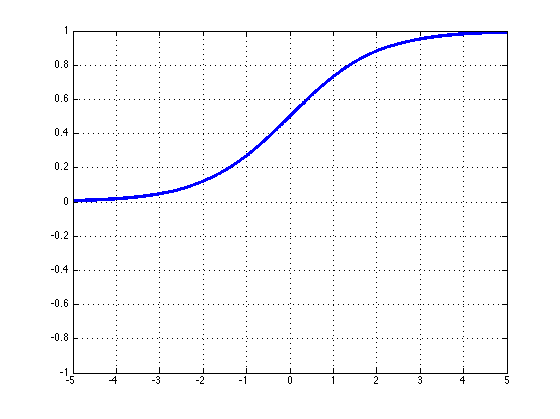
\includegraphics[width=0.5\textwidth]{images/eman/graph_sigmoid.png}
  \caption[The response of a sigmoid nonlinearity ]{The response of a sigmoid nonlinearity}
  \label{fig:graph_sigmoid}
\end{figure}
\textbf{Tanh:}\\ 
The tanh function is an alternative to the sigmoid function that is often found to converge faster in practice. The primary difference between tanh and sigmoid is that tanh output ranges from $-1$ to $1$ while the sigmoid ranges from $0$ to $1$.
\begin{align*}
  \operatorname{tanh}(z) &=  \frac{\operatorname{exp}(z) - \operatorname{exp}(-z)}{\operatorname{exp}(z) + \operatorname{exp}(-z)} = 2\sigma(2z) - 1\\
  \text{where}~\operatorname{tanh}(z) &\in (-1, 1)
\end{align*}
The gradient of $ \operatorname{tanh}(z) $ is:
$$ \operatorname{tanh}'(z) = 1 - \bigg(\frac{\operatorname{exp}(z) - \operatorname{exp}(-z)}{\operatorname{exp}(z) + \operatorname{exp}(-z)}\bigg)^2 = 1 - \operatorname{tanh}^2(z)$$
\begin{figure}[H]%
  \center%
    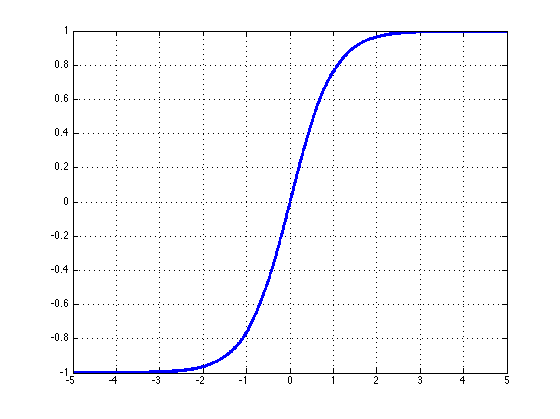
\includegraphics[width=0.5\textwidth]{images/eman/graph_tanh.png}
  \caption[The response of a tanh nonlinearity ]{The response of a tanh nonlinearity}
  \label{fig:graph_tanh}
\end{figure}
\textbf{Soft sign:}
The soft sign function is another nonlinearity which can be considered an alternative to tanh since it too does not saturate as easily as hard clipped functions:
$$\operatorname{softsign}(z) = \frac{z}{1 + |z|}$$
The derivative is the expressed as:
$$\operatorname{softsign}'(z) = \frac{\operatorname{sgn}(z)}{(1 + z)^2}$$
$$\text{where}~\operatorname{sgn} \text{ is the signum function which returns }\pm1\text{ depending on the sign of }z$$
\begin{figure}[H]%
  \center%
    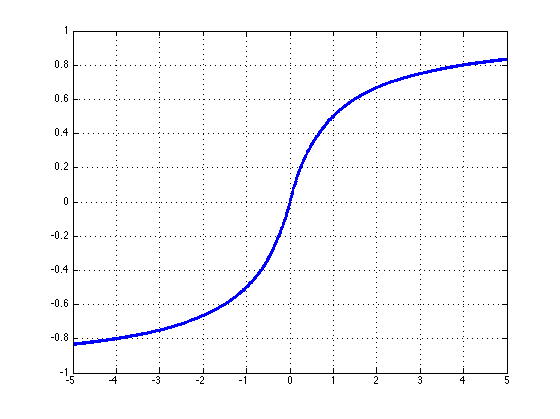
\includegraphics[width=0.5\textwidth]{images/eman/graph_softsign.png}
  \caption[The response of a soft sign nonlinearity]{The response of a soft sign nonlinearity}
  \label{fig:graph_softsign}
\end{figure}
\textbf{ReLU:} The ReLU (Rectified Linear Unit) function is a popular choice of activation since it does not saturate even for larger values of $z$ and has found much success in computer vision applications:
$$\operatorname{rect}(z) = \operatorname{max}(z, 0)$$
The derivative is then the piecewise function:
\begin{displaymath}
    \operatorname{rect}'(z) = \left\{
     \begin{array}{cl}
       1 & : z > 0\\
       0 & : \text{otherwise}
     \end{array}
   \right.
\end{displaymath}
\begin{figure}[H]%
  \center%
    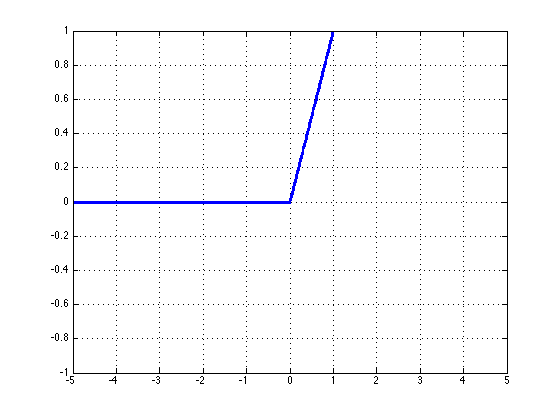
\includegraphics[width=0.5\textwidth]{images/eman/graph_relu.png}
  \caption[The response of a ReLU nonlinearity]{The response of a ReLU nonlinearity}
  \label{fig:graph_relu}
\end{figure}
\textbf{Leaky ReLU:} Traditional ReLU units by design do not propagate any error for non-positive $z$ -- the leaky ReLU modifies this such that a small error is allowed to propagate backwards even when $z$ is negative:
$$\operatorname{leaky}(z) = \operatorname{max}(z, k\cdot z)$$
$$\text{where } 0<k<1$$
This way, the derivative is representable as:
\begin{displaymath}
    \operatorname{leaky}'(z) = \left\{
     \begin{array}{cl}
       1 & : z > 0\\
       k & : \text{otherwise}
     \end{array}
   \right.
\end{displaymath}
\begin{figure}[H]%
  \center%
    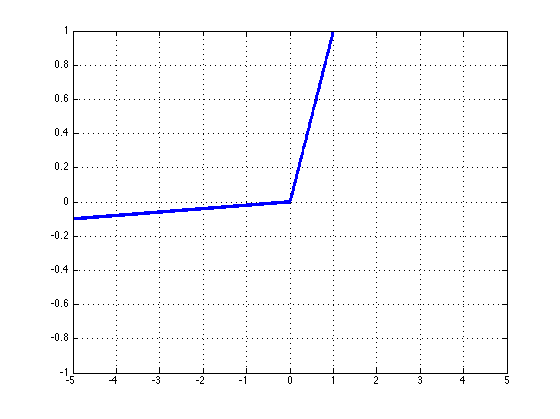
\includegraphics[width=0.5\textwidth]{images/eman/graph_leaky.png}
  \caption[The response of a leaky ReLU nonlinearity]{The response of a leaky ReLU nonlinearity}\label{fig:graph_leaky}
\end{figure}
\subsection{Adam optimization algorithm?}
Adam is an optimization algorithm that can used instead of the classical stochastic gradient descent procedure to update network weights iterative based in training data.
\subsection{AdaGrad algorithm?}
AdaGrad is an optimization method that allows different step sizes for different features. It increases the influence of rare but informative features.






